\documentclass{article}
\usepackage{graphicx}
\usepackage{amsmath}
\usepackage{pgfplots}
\usepackage{physics}
\usepackage{cancel}
\usepackage{bigints}
\usepackage{enumitem}
\usepackage{txfonts}
\usepackage[normalem]{ulem}

\newcommand{\g}{\text{g}}
\newcommand{\kilo}{\text{k}}
\newcommand{\m}{\text{m}}
\newcommand{\centi}{\text{c}}
\newcommand{\s}{\text{s}}
\newcommand{\N}{\text{N}}
\newcommand{\J}{\text{J}}
\newcommand{\C}{\text{C}}
\newcommand{\V}{\text{V}}
\newcommand{\A}{\text{A}}
\newcommand{\Ohm}{\text{\Omega}}
\newcommand{\p}{\text{p}}

\pgfplotsset{compat=1.18}

\pgfplotsset{compat=1.18}

\usepackage[a4paper, top=1cm, bottom=2cm, left=2cm, right=2cm, includehead, includefoot]{geometry}



\begin{document}

\noindent
Physics 4B - Electromagnetism \hfill Prof. Alfred Cauthen
\noindent\rule{\textwidth}{0.4pt}

\begin{center}
    \textbf{\LARGE Homework 8} \\
    \vspace{12pt}
    \large Aaron W. Tarajos \\
    \textit{\today}
\end{center}

\noindent\rule{\textwidth}{0.4pt}

\section*{Chapter 3 Problem 73}
Two vectors are given by $\vec{a} = 3.0\hat{i} + 5.0\hat{j}$ and $\vec{b} = 2.0\hat{i} + 4.0\hat{j}$.
Find (a) $\vec{a} \times \vec{b}$, 
(b) $\vec{a} \cdot \vec{b}$, 
(c) $(\vec{a} + \vec{b}) \cdot \vec{b}$, and
(d) the component of $\vec{a}$ along the direction of $\vec{b}$.

\subsection*{Solution}
\textbf{Part a:}

\begin{align*}
\vec{a} \times \vec{b} &= \begin{vmatrix}
    \hat{i} & \hat{j} & \hat{k} \\
    3.0 & 5.0 & 0 \\
    2.0 & 4.0 & 0
\end{vmatrix} \\ 
&= \hat{k}(3.0 \cdot 4.0 - 5.0 \cdot 2.0) \\
&= \hat{k}(12.0 - 10.0) \\
&= \boxed{2.0\hat{k}}
\end{align*}
\textbf{Part b:}

\begin{align*}
\vec{a} \cdot \vec{b} &= 3.0 \cdot 2.0 + 5.0 \cdot 4.0 \\
&= 6.0 + 20.0 \\
&= \boxed{26.0}
\end{align*}
\textbf{Part c:}

\begin{align*}
(\vec{a} + \vec{b}) \cdot \vec{b} &= (3.0\hat{i} + 5.0\hat{j} + 2.0\hat{i} + 4.0\hat{j}) \cdot (2.0\hat{i} + 4.0\hat{j}) \\
&= (5.0\hat{i} + 9.0\hat{j}) \cdot (2.0\hat{i} + 4.0\hat{j}) \\
&= 10.0 + 36.0 \\
&= \boxed{46.0}
\end{align*}
\textbf{Part d:}

\begin{align*}
\text{comp}_{a}\vec{b} &= \frac{\vec{a} \cdot \vec{b}}{b} \\
&= \frac{26.0}{\sqrt{2.0^2 + 4.0^2}} \\
&= \boxed{\frac{26.0}{\sqrt{20.0}}}
\end{align*}

\section*{Chapter 21 Problem 21}
A nonconducting spherical shell, with an inner radius of 4.0 cm and an outer radius of 6.0 cm, has charge spread nonuniformly through its volume between its inner and outer surfaces.
The volume charge density $\rho$ is the charge per unit volume, with the unit coulomb per cubic meter. For this shell $\rho = b/r$, where $r$ is the distance in meters from the center of the shell and $b = 3.0 \mu C/m^2$.
What is the net charge in the shell?

\subsection*{Solution}

\begin{align*}
    \rho &= \frac{dQ}{dV} \\
    dQ &= \rho dV \\
    \int dQ &= \int \rho dV \\
    Q &= \int \frac{b}{r} dV \\
    Q &= \int \frac{b}{r} 4\pi r^2 dr \\
    &= 4\pi b \int_4^6 r dr \\
    &= 4\pi b \left[\frac{r^2}{2}\right]_4^6 \\
    &= 4\pi b \left(\frac{36}{2} - \frac{16}{2}\right) \\
    &= 4\pi b \left(18 - 8\right) \\
    &= 4\pi b \cdot 10 \\
    &= 40\pi b \\
    &= 40\pi (3.0 \times 10^{-6}) \\
    &= \boxed{120\pi\ \mu \C}
\end{align*}

\section*{Chapter 22 Problem 30}
Figure 22-53 shows two concentric rings, of radii $R$ and $R^\prime = 3.00R$, that lie on the same plane. 
Point $P$ lies on the central axis, at distance $D = 2.00R$ from the center of the rings. 
The smaller ring has uniformly distributed charge $Q$. 
In terms of $Q$, what is the uniformly distributed charge on the larger ring if the net electric field at $P$ is zero?

\begin{figure}[h]
    \centering
    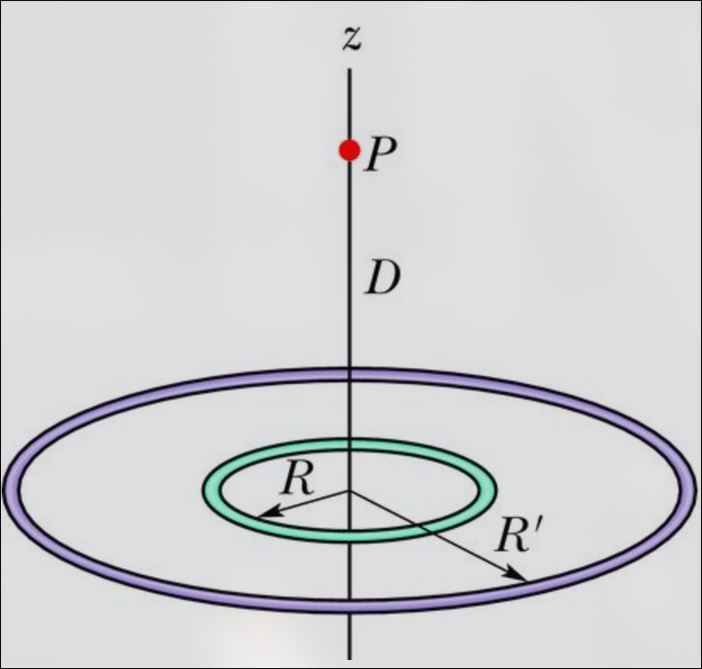
\includegraphics[width=0.5\textwidth]{image-1.png}
    \caption{Figure 22-53}
\end{figure}

\subsection*{Solution}
\[
\vec{E}_{net} = \vec{E}_R + \vec{E}_R^\prime = 0
\]
where $\vec{E}_R$ is the electric field due to the smaller ring and $\vec{E}_R^\prime$ is the electric field due to the larger ring given by;
\[
E_R = \frac{kQ}{R^2 + D^2}
\]
and

\[
E_R^\prime = \frac{kQ^\prime}{R^{\prime2} + D^2}
\]
so we have;
\begin{align*}
    \frac{kQ}{R^2 + D^2} &= -\frac{kQ^\prime}{R^{\prime2} + D^2} \\
    Q^\prime &= -Q \frac{R^2 + D^2}{R^{\prime2} + D^2} \\
    &= -Q \frac{R^2 + (2.00R)^2}{(3.00R)^2 + (2.00R)^2} \\
    &= -Q \frac{R^2 + 4.00R^2}{9.00R^2 + 4.00R^2} \\
    &= -Q \frac{5.00R^2}{13.00R^2} \\
    &= -\frac{5.00}{13.00}Q \\
    &= \boxed{-\frac{5}{13}Q}
\end{align*}

\section*{Chapter 23 Problem 42}
Two large metal plates of area 1.0 m2 face each other,
5.0 cm apart, with equal charge magnitudes $|q|$ but opposite
signs. The field magnitude $E$ between them
(neglect fringing) is 55 N/C. Find $|q|$.

\subsection*{Solution}
The field from one of the plates is given by;
\[
E = \frac{\sigma}{2\varepsilon_0}
\]
and so we have;
\begin{align*}
    \vec{E}_{net} &= \vec{E}_1 + \vec{E}_2 \\
    55 &= \frac{\sigma}{2\varepsilon_0} + \frac{\sigma}{2\varepsilon_0} \\
    55 &= \frac{\sigma}{\varepsilon_0} \\
    \sigma &= 55 \varepsilon_0 \\
    \frac{q}{A} &= 55 \varepsilon_0 \\
    q &= 55 \varepsilon_0 A \\
    &= 55 (8.85 \times 10^{-12}) (1.0) \\
    &= 4.86 \times 10^{-10} C \\
    &= \boxed{486\ \text{pC}}
\end{align*}

\section*{Chapter 24 Problem 37}
What is the magnitude of the electric field at the point
$(3.00\vu{i} - 2.00\vu{j} + 4.00\vu{k}) \m$ if the electric potential in the region is
given by $V = 2.00xyz^2$, where $V$ is in volts and coordinates $x$, $y$, and
$z$ are in meters?

\subsection*{Solution}
\begin{align*}
    \vec{E} &= -\nabla V \\
    &= -\left(\frac{\partial V}{\partial x} \vu{i} + \frac{\partial V}{\partial y} \vu{j} + \frac{\partial V}{\partial z} \vu{k}\right)\\
    &= -\left(\frac{\partial}{\partial x}\left[2.00xyz^2\right] \vu{i} + \frac{\partial}{\partial y}\left[2.00xyz^2\right] \vu{j} + \frac{\partial}{\partial z}\left[2.00xyz^2\right] \vu{k}\right)\\
    &= -2.00yz^2\ \vu{i} - 2.00xz^2\ \vu{j} - 4.00xyz\ \vu{k} \\
    &= -2.00(-2)(4)^2\ \vu{i} - 2.00(3)(4)^2\ \vu{j} - 4.00(3)(-2)(-2)\ \vu{k} \\
    &= \boxed{64\ \vu{i} - 96\ \vu{j} + 48\ \vu{k}}
\end{align*}

\section*{Chapter 24 Problem 64}
A hollow metal sphere has a potential of $+400 \V$ with respect
to ground (defined to be at $V = 0$) and a charge of $5.0 \times 10^{-9}\ \C$. Find
the electric potential at the center of the sphere.

\subsection*{Solution}
Its a sphere, therefore the potential is the same everywhere.
\[
    \boxed{V = 400\V}
\]

\section*{Chapter 24 Problem 67}
A metal sphere of radius $15\ \centi \m$ has a net charge of
$3.0 \times 10^{-8}\ \C$. (a) What is the electric field at the sphere’s surface?
(b) If $V = 0$ at infinity, what is the electric potential at the sphere’s
surface? (c) At what distance from the sphere’s surface has the
electric potential decreased by $500 \V$?

\subsection*{Solution}
\textbf{Part a:}

\begin{align*}
    E &= \frac{kQ}{r^2} \\
    &= \frac{(8.99 \times 10^9)(3.0 \times 10^{-8})}{(0.15)^2} \\
    &= \boxed{1.2 \times 10^4\ \text{N/C}}
\end{align*}
\textbf{Part b:}

\begin{align*}
    V &= -\int_\infty^r E dr \\
    &= -\int_\infty^{0.15} \frac{(8.99 \times 10^9)(3.0 \times 10^{-8})}{r^2} dr \\
    &= \frac{(8.99 \times 10^9)(3.0 \times 10^{-8})}{0.15} \\
    &= \boxed{1.8 \times 10^3\ \text{V}}
\end{align*}
\textbf{Part c:}

\begin{align*}
    V &= -\int_\infty^r E dr \\
    1.8 \times 10^3 &= -\int_\infty^r \frac{(8.99 \times 10^9)(3.0 \times 10^{-8})}{r^2} dr \\
    &= \frac{(8.99 \times 10^9)(3.0 \times 10^{-8})}{r} \\
    &= \boxed{0.06\ \text{m}}
\end{align*}

\section*{Chapter 25 Problem 1}
The two metal objects in Fig. 25-24 have net charges of
$+70\ \p\C$ and $-70\ \p\C$, which result in a $20\ \V$ potential difference
between them. (a) What is the capacitance of the system? (b) If the
charges are changed to $+200\ \p\C$ and $-200\ \p\C$, what does the capacitance become? (c) What does the potential difference become?

\begin{figure}[h]
	\centering
	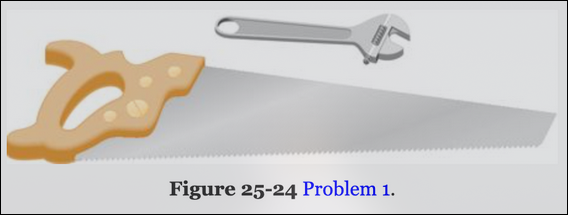
\includegraphics[width=0.5\textwidth]{image-2.png}
	\caption{Figure 25-24}
\end{figure}

\subsection*{Solution}
\textbf{Part a:}

\begin{align*}
    C &= \frac{Q}{V} \\
    &= \frac{70 \times 10^{-12}}{20} \\
    &= \boxed{3.5 \times 10^{-11}\ \text{F}}
\end{align*}
\textbf{Part b:}

\begin{align*}
    C &= \frac{Q}{V} \\
    &= \frac{200 \times 10^{-12}}{20} \\
    &= \boxed{10 \times 10^{-11}\ \text{F}}
\end{align*}
\textbf{Part c:}

\begin{align*}
    V &= \frac{Q}{C} \\
    &= \frac{200 \times 10^{-12}}{3.5 \times 10^{-11}} \\
    &= \boxed{5.71\ \text{V}}
\end{align*}

\end{document}